\chapter{Software de adquisición}
\label{cap2}
En este capítulo procedemos a explicar el funcionamiento del software de adquisición. Empezaremos recordando los aspectos básicos descritos en el
capítulo de introducción. El funcionamiento nominal del software consiste en recoger la información de los módulos hardware como la FPGA, el
barómetro, las fuentes de alimentación y los sensores de temperatura si estos están presentes. Cada minuto, la información recogida es procesada y
almacenada en una base de datos. 
\par
Antes de empezar a discutir a fondo el software de adquisición es conveniente estar familiarizados con el entorno hardware descrito en el capítulo
\ref{entornoHW}. El software es ejecutado en la \emph{BeagleBone Black} sobre un Linux, distribución \emph{Angstrom}. El lenguaje elegido para el desarrollo es
\emph{Python}\cite{Python}. Este  es un lenguaje interpretado de alto nivel con una sintaxis centrada en producir un código legible. El lenguaje se adapta
igualmente bien a programación imperativa y orientada a objetos. El tipado dinámico da mucha flexibilidad al lenguaje. Todas estas propiedades del
lenguaje permiten un desarrollo rápido. Además el lenguaje ofrece una amplia cantidad de bibliotecas que también aligeran el trabajo. 
\par
Para gestionar la base de datos utilizamos \emph{Sqlite3}\cite{Sqlite}. Este es un gestor muy ligero y adecuado para sistemas empotrados. Aparte de esta base
de datos local, el software permite mantener una segunda réplica remota. Para esta réplica remota utilizamos \emph{MySql}\cite{MySql} que es un gestor más
completo con enfoque \emph{Cliente-Servidor}.
\par
En la figura \ref{fig:soft_adquisición} podemos ver un diagrama de flujo que describe el funcionamiento de nuestro software. A lo largo de este
capítulo haremos muchas referencias a este diagrama para explicar los diferentes módulos software que lo componen. Podemos ver que hay cuatro módulos
principales, a continuación hacemos una breve descripción de estos. 
\begin{itemize}
  	\item	\texttt{NMDA}. Es el proceso principal de nuestro software. Es el encargado de realizar las configuraciones necesarias e iniciar
	  	el \texttt{FPGASerialReader} y el \texttt{CountsManager}.
	\item	\texttt{FPGASerialReader}. \emph{Thread} que se encarga de procesar la información transmitida por la FPGA.
	\item	\texttt{CountsManager}. \emph{Thread} que se enarga de pedir la información necesaria y guardarla en la base de datos con periodicidad
	  	de un minuto. Después de guardar la información es iniciado el \texttt{DBUpdater}.
	\item	\texttt{DBUpdater}. \emph{Thread} que se encarga de sincronizar la base de datos local con la réplica remota.
\end{itemize}

\begin{sidewaysfigure}[p]
	\centering
	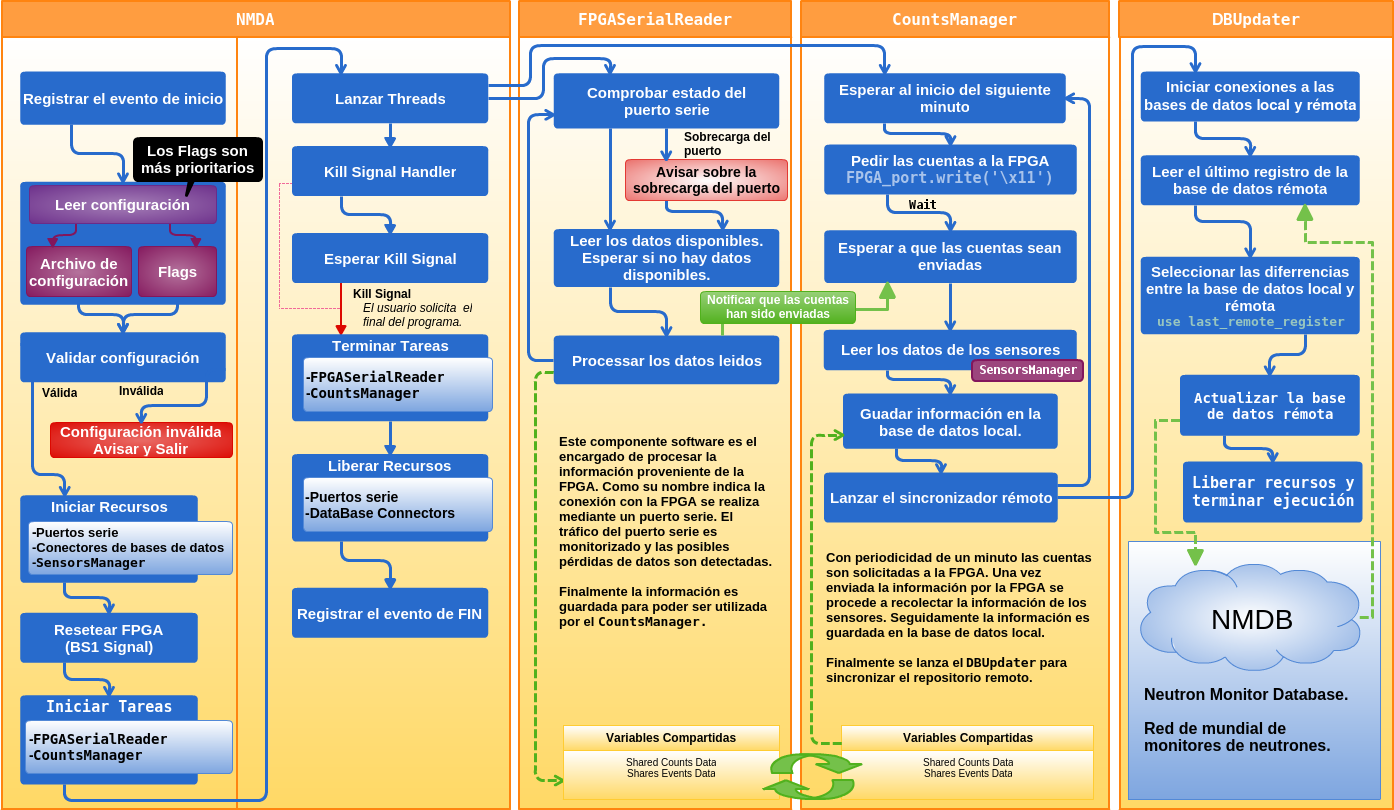
\includegraphics[keepaspectratio, width=1\textwidth]{./img/soft_adquisicion.png}
	\caption{Diagrama de flujo. Software de adquisición.}
	\label{fig:soft_adquisición}
\end{sidewaysfigure}

\section{Arranque automático del sistema}
	Uno de los requisitos del sistema es el arranque automático ante la presencia de corriente eléctrica. La \emph{BeagleBone Black} por defecto está
	configurada para arrancar automáticamente,pero debemos configurarla para que también inicialice nuestro software. Para este propósito vamos a
	utilizar las \emph{System Services}\cite{AngSystemctl} que \emph{Angstrom} proporciona. Esta distribución utiliza \texttt{systemd}\cite{systemdWiki}
	para gestionar los servicios de sistema y la forma en la que estos servicios arrancan cuando se pone en marcha la \emph{BeagleBone Black}. Este es un
	conjunto de demonios, bibliotecas y utilidades diseñados para facilitar la administración de sistemas Linux.
	\par
	Para operar sobre la configuración de \texttt{systemd} tenemos el comando \texttt{systemctl}. A continuación podemos ver como usar este
	comando.
	\begin{lstlisting}[style=myBash]
$ systemctl start    nombre_de_servicio
$ systemctl restart  nombre_de_servicio
$ systemctl stop     nombre_de_servicio
$ systemctl status   nombre_de_servicio
$ systemctl enable   nombre_de_servicio
$ systemctl disable  nombre_de_servicio
	\end{lstlisting}
	\par
	Los servicios de sistema se crean mediante archivos con extensión \texttt{.service} que deben ser guardados en el directorio
	\texttt{/lib/systemd/system}. En el apéndice \ref{appendix:systemctl} podemos ver el contenido de los archivos que definen los cuatro
	servicios de sistema utilizados en este trabajo. Veamos el significado de lo campos más importantes que son definidos en estos archivos.
	\begin{itemize}
		\item	\texttt{Description}. Un mensaje descriptivo del servicio. Permite al usuario entender el propósito de este de forma fácil.
		\item	\texttt{Before} y \texttt{After}. Estos dos campos pueden referenciar a otros servicios para indicar que este debe ejecutarse
			antes o después del servicio que es citado. Esto permite definir un orden en el que serán ejecutados los servicios de sistema.
			También es posible especificar un grupo de servicios como el \texttt{network.target} que agrupa los servicios responsables de
			establecer la conexión a Internet. 
		\item	\texttt{Type}. El tipo del servicio. Con este campo podemos dar diferentes propiedades a nuestro servicio. Los valores
			aceptados que utilizamos son \texttt{oneshot}, \texttt{forking} y \texttt{simple}, que es el valor por defecto.
		\item	\texttt{ExecStart}. El comando y argumentos que queremos ejecutar.
		\item	\texttt{WantedBy}. Es el grupo al que este servicio pertenece. El grupo \texttt{multi-user.target} es un grupo para los
			servicios de un sistema multiusuario. Este campo hace que este servicio sea retrasado hacia el final del proceso de arranque,
			específicamente hasta que el sistema sea listo para aceptar el acceso de múltiples usuarios. 
	\end{itemize}
	\par
	En la figura \ref{fig:boot} podemos ver la secuencia que define el proceso de arranque del sistema de adquisición. Esta secuencia empieza con
	el servicio \texttt{myWatchDog.service}, que es el encargado de arrancar el software que controla el \emph{Watchdog}. El servicio
	\texttt{ntpdate.service} es el responsable de establecer la fecha y hora actuales mientras que el servicio \texttt{ntpd.service} tiene como
	tarea corregir las derivas que pueden presentrase. Finalmente el servicio \texttt{nmda.service} es el encargado de arrancar el software de
	adquisición.
	\begin{figure}[h]
		\centering
		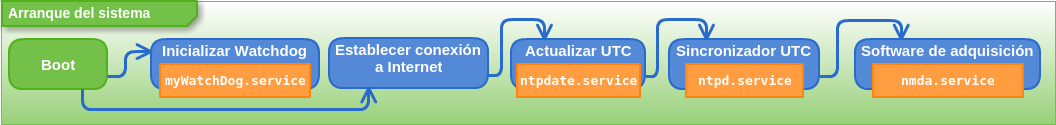
\includegraphics[keepaspectratio, width=1\textwidth]{./img/boot.png}
		\caption{Arranque del sistema}   
		\label{fig:boot}
	\end{figure}
	\subsection{Watchdog}
		Un \emph{Watchdog} \cite{WatchDogWiki} es un mecanismo de seguridad que realiza un \emph{Reset} en el sistema cuando es detectado un mal
		funcionamiento. Consiste en un temporizador que realiza una cuenta atrás, de forma que, cuando esta cuenta llega a cero, el sistema es
		reiniciado. Es nuestro software el que debe reponer el valor de este contador para evitar que expire. Los \emph{Watchdogs} pueden ser
		software o hardware, el utilizado en este trabajo está implementado en la \emph{BeagleBone Black} y es hardware. Los \emph{Watchdogs} hardware son
		más fiables, los software son más susceptibles a bloquearse.
		\par
		El \emph{Watchdog} es accesible mediante el archivo \texttt{/dev/watchdog}. Para activar el mecanismo basta con escribir cualquier valor en
		dicho archivo. El contador se pone en marcha automáticamente y, si este llegara a expirar, se produciría el reinicio del sistema. El
		valor inicial del contador es de 60 segundos, valor que adquiere cada vez que es reiniciado. El contador es reiniciado al volver a
		escribir en el archivo. Al cerrar dicho archivo el mecanismo es deshabilitado. A continuación presentamos una parte del código fuente
		responsable de controlar el \emph{WatchDog}.
		\begin{lstlisting}[style=myPython]
args		= NMDA.create_parser().parse_args()
conn_local      = sqlite3.connect(args.database)
last_data       = get_last()
cont            = 0

wd = open("/dev/watchdog", "w+")
while True:
    time.sleep(20)
    wd.write("\n")
    wd.flush()
    cont+=1

    if cont >= 15:            #15*20secs=5mins
        cont            = 0
        curr_last       = get_last()
        if curr_last == last_data:
            time.sleep(120)   #Este sleep reinicia la placa
        last_data       = curr_last
		\end{lstlisting}
		\par
		Primero se establece la conexión con la base de datos local. La base de datos es utilizada para comprobar si el sistema de adquisición
		genera correctamente datos. Si no fuera así, la placa debe ser reiniciada. Una vez establecida la conexión se procede a invocar la
		función \texttt{get\_last()}, que devuelve el último valor presente en la base de datos. Seguidamente se abre el archivo que permite
		manejar el \emph{WatchDog}. Una vez abierto el archivo se entra en un bucle \texttt{while} sin condición de salida. En cada iteración de este
		bucle se escribe un salto de línea que reinicia el contador del \emph{WatchDog}. Dentro del bucle también hay una llamada a la función
		\texttt{time.sleep(20)}, las iteraciones del bucle están espaciadas 20 segundos. Cada 15 iteraciones o aproximadamente 5 minutos se
		vuelve a invocar la función \texttt{get\_last()}. El valor devuelto es comparado con el valor anterior. Si estos dos valores son
		iguales es invocada la función \texttt{time.sleep(120)}, intervalo suficiente para que el contador del \emph{WatchDog} expire. Los valores
		son iguales si en los últimos 5 minutos el sistema de adquisición no ha generado ningún dato. Por contrario si se han generado datos
		durante los últimos 5 minutos estos dos valores son diferentes, en tal caso se sigue con la ejecución del bucle \texttt{while}. 
	\subsection{Sincronización de fecha y hoara}
		La \emph{BeagleBone Black} no implementa ningún mecanismo hardware para mantener la fecha y hora actuales, por lo que en cada reinicio la
		fecha y hora se pierden. Es nuestra responsabilidad realizar un mecanismo software que sincronice la fecha y hora con el resto del
		mundo\cite{ntpd}. Utilizamos el programa \texttt{ntpd} para este propósito. Este programa hace uso del \emph{Network Time
		Protocol}\cite{ntpWiki}, que permite la sincronización entre dos relojes a través de una red de datos con latencia variable. Son
		realizadas dos llamadas a este programa.
		\begin{lstlisting}[style=myBash]
# Establece inicialmente la fecha y hora.
$ /usr/bin/ntpd -q -g -x
# Lanza un demonio que corrige las derivas que puedan presentarse
$ /usr/bin/ntpd -p /run/ntpd.pid
		\end{lstlisting}

\section{\texttt{NMDA}}
	Este es el módulo principal de nuestro software. Es el encargado de realizar la configuración inicial de acuerdo con los parámetros
	proporcionados, resetear la FPGA y finalmente inicializar los demás módulos. En la figura \ref{fig:soft_adquisición} podemos ver un diagrama
	de flujo que representa el funcionamiento de este. En las siguientes subsecciones describiremos las funcionalidades más relevantes de este
	módulo.
	\subsection{Logger}
		Haciendo uso de la biblioteca \texttt{logging}\cite{py_logging} se configura un archivo de Log. En este archivo se registran los sucesos
		de eventos importantes. Un ejemplo de los posibles eventos que se registran son los relacionados con las pérdidas de datos. El
		mecanismo está configurado para que automáticamente se guarde la hora y fecha de cada mensaje. A continuación se muestra cómo se
		configura y usa este mecanismo. Los comentarios representan la entrada producida en el archivo de Log.
		\begin{lstlisting}[style=myPython]
import logging
logging.basicConfig(filename='/server/logs/NMDA.log', level=logging.DEBUG, format=''%(asctime)s %(message)s'')
logging.info('Data Loss')   
# 2015-05-14 09:50:56,017   Data Loss
logging.info('Uart_1 Overflow') 
# 2015-05-14 09:50:55,936   Uart_1 Overflow
		\end{lstlisting}
	\subsection{Archivo de configuración y Flags}
		Existen una serie de parámetros que varían en función de la estación o que simplemente pueden cambiar con el tiempo. No es buena idea
		tener los valores de estas variables en el código. Este problema nos ha llevado a exportar estos parámetros a un archivo de
		configuración. Para leer este archivo utilizamos la biblioteca \texttt{ConfigParser}\cite{py_ConfigParser}. A continuación mostramos un
		ejemplo de este archivo que nos ayudará a entender mejor su estructura. Los comentarios explicativos son suficientes para entender el
		propósito de cado uno de los campos.
		\begin{lstlisting}[style=myFile]
[Basics]
# Referencia a la Uart de pulsos dentro del sistema de archivos.
serial_port_control  = /dev/ttyO2
# Referencia la la base de datos local.
# El valor 'shell' imprimirá los valores por consola.
database = /server/data/test.db
# Valores medios para los 18 canales que serán utilizados para el Median Algorithm.
Channel_avg = 255, 290, 0, 295, 0, 0, 289, 291, 252, 254, 293, 299, 298, 328, 299, 302, 302, 272

[Sensors]
# Referencia a la Uart de extensión dentro del sistema de archivos.
serial_port_sensors= None
# Tipo de barómetro. Valores aceptados [None, bm35, ap1].
barometer_type = None
# Tipo de HVPS. Valores acpetados [None, analog, digital].
hvps_type = None
# Coeficiente de correción para las HVPS analógicas.
analog_hvps_corr = 1.0

[dbUpdater]
# Habilitar y deshabilitar.
db_updater_enabled=True
# Referencia la la base de datos local. Debe tener el mismo valor que Basics.database.
local_db= /server/data/test.db 
# La dirreción IP de la base de datos remota.
remote_db_host= 192.168.1.1
# Usuario y contraseña del usuario para la base de datos remota
remote_db_user= hristo
remote_db_pass= 123qwe
# Nombre de la base de datos remota
remote_db_db= nmdadb2

[Pressure]
# Presión media para la estación
avg_pressure=932
# Coeficiente de correlación atmosférica
beta_pressure=0.0067

[Efficiency]
# Factor de correción
beta_efficiency=1.0
\end{lstlisting} 
		\par
		Los valores de los parámetros exportados son también accesibles a través de flags. En este caso hemos utilizado la biblioteca
		\texttt{argparse}\cite{py_argparse}. Los valores especificados mediante flags tienen precedencia sobre los mismos que estuvieran en el
		archivo de configuración. Los flags se usan de la siguiente forma.
		\newpage
		%\enlargethispage{-1\baselineskip}
		\begin{lstlisting}[style=myBash]
$ python NMDA.py -h
usage: NMDA.py 
   [-h] [-sp SERIAL_PORT_CONTROL] [-db DATABASE]
   [-sps SERIAL_PORT_SENSORS] [-bm {ap1,bm35}]
   [-hv {digital,analog}] [-ahvc ANALOG_HVPS_CORR]
   [-dbU DB_UPDATER_ENABLED] [-ldb LOCAL_DB] [-rh REMOTE_DB_HOST]
   [-ru REMOTE_DB_USER] [-rp REMOTE_DB_PASS] [-rdb REMOTE_DB_DB]
   [-apr AVG_PRESSURE]
		\end{lstlisting}

	\subsection{Configurar la BeagleBone Black}
		Tal y como explicamos en el capítulo de entorno hardware la \emph{BeagleBone Black} proporciona dos conectores de expansión de 46 pines cada
		uno\cite{BeagleWikiExp}. Muchos de estos pines son multipropósito, es decir, que están compartidos por varias unidades funcionales
		internas, por lo que debe configurarse a cuál de ellas se conectará. Esta configuración se realiza mediante el uso de \emph{Device
		Tree Overlay}, que es una estructura de datos utilizada para describir el hardware.
		\par
		En este trabajo utilizamos la biblioteca \emph{Adafruit BeagleBone IO Python}\cite{AdaFruitGit} que facilita la tarea de configurar
		estas cabeceras. A continuación podemos ver una lista de los pines utilizados y la función de cada uno en el ámbito de este proyecto.
		\begin{lstlisting}[style=myBash]
Pin P9_21(UART2_TXD) --> Uart de Control trasmisión
Pin P9_22(UART2_RXD) --> Uart de Control recepción
Pin P9_24(UART1_TXD) --> Uart de Extensión trasmisión
Pin P9_26(UART1_RXD) --> Uart de Extensión recepción
Pin P9_37(AIN2)	     --> Entrada analógica(sensores analógicos)
Pin P9_38(AIN3)	     --> Entrada analógica(sensores analógicos)
Pin P9_39(AIN0)	     --> Entrada analógica(sensores analógicos)
Pin P9_40(AIN1)	     --> Entrada analógica(sensores analógicos)
Pin P9_42(GPIO_7)    --> Reset de la FPGA.
Pin P8_08(GPIO_67)   --> Señal DATA del barómetro AP1.
Pin P8_09(GPIO_69)   --> Señal CLOCK del barómetro AP1.
Pin P8_10(GPIO_68)   --> Señal STROBE del barómetro AP1.
		\end{lstlisting}

	\subsection{Iniciar recursos}
		Al ser el módulo principal, \texttt{NMDA} es el encargado de iniciar todos los recursos que serán utilizados. Por recursos nos
		referimos a las variables compartidas entre \emph{threads}, conectores a las bases de datos, interfaces de los puertos serie y otros.
		Para los conectores a las bases de datos utilizamos las bibliotecas \texttt{sqlite3} y \texttt{MySQLdb}, volvemos a recordar que tenemos
		una réplica local con \emph{Sqlite3} y otra réplica remota que gestionamos con \emph{MySql}. Las tablas son creadas automáticamente en caso de no
		existir, esto simplifica mucho el proceso de implantación. Para la interfaz de los puertos serie utilizamos la biblioteca
		\texttt{serial}.
		\par
		Son inicializados los otros dos \emph{threads}, \texttt{FPGASerialReader} y \texttt{CountsManager}. Estos dos realizan todo el proceso
		de adquisición y serán descritos más adelante en este capítulo. 
	\subsection{Resetear FPGA}
		Como hemos explicado en el capítulo \ref{entornoHW}, la FPGA permite realizar un \emph{Reset}, que el software realizará antes de empezar con
		la adquisición de datos. Este \emph{Reset} asegura que la FPGA está en un correcto estado. Para realizar el \emph{Reset} utilizamos la señal
		digital, \emph{BS1}, que está conectada al pin \emph{P9\_42} de la \emph{BeagleBone Black}. Volvemos a recordar que esta es activa a nivel
		bajo. Para controlarla utilizaremos la biblioteca de \emph{AdaFruit}\cite{AdaFruitGit}, que gestiona las entradas y salidas de propósito
		general(GPIO) de la siguiente forma.
		\begin{lstlisting}[style=myPython]
import Adafruit_BBIO.GPIO as GPIO
GPIO.setup('P9_42', GPIO.OUT)
GPIO.output('P9_42', GPIO.LOW)
time.sleep(0.5)
GPIO.output('P9_42', GPIO.HIGH)
		\end{lstlisting}
	
	\subsection{Kill Signal Handler}
		Este es un software que debe ejecutarse indefinidamente. En su uso real no será interrumpido, pero hemos implementado un mecanismo que
		permite pararlo. Este mecanismo permite solicitar el fin del programa, que desencadena una serie de acciones. Estas acciones tienen
		como objetivo asegurar que todos los recursos sean liberados de forma correcta. Liberar los recursos de forma correcta supone no tener
		ningún conflicto si seguidamente volvemos a ejecutar el software. Esto en el uso real del software no tiene gran impacto, sin embargo
		ha sido muy útil durante el proceso de desarrollo.

\section{\texttt{FPGASerialReader}}
	Este módulo software es el encargado de leer y procesar los datos transmitidos por la FPGA. En la figura \ref{fig:soft_adquisición} podemos
	ver un diagrama de flujo que refleja el funcionamiento de este. La ejecución del \emph{thread} empieza comprobando el estado del puerto serie,
	que puede estar saturándose. En el caso de que el puerto esté saturado se genera una entrada en el archivo de Log indicando este hecho. A
	continuación leemos los datos disponibles, y en caso de no haber datos disponibles el \emph{thread} se queda bloqueado esperando a la llegada
	de estos. Seguidamente de leer los datos pasamos a procesarlos. Por procesar nos referimos a interpretar el significado que tienen. Finalmente
	volvemos al paso inicial, volviendo a comprobar si han llegado nuevos datos a la UART.
	\par
	En las tablas \ref{tab:FPGAUartPulso}, \ref{tab:FPGAUartOver} y \ref{tab:FPGAUartCont}  del capítulo \ref{entornoHW}, podemos ver el formato
	de los datos que tenemos que procesar. Vemos que hay tres tipos de mensajes que podemos recibir. Los mensajes no siguen un orden concreto,
	además llegan de forma totalmente asíncrona. Además el canal de trasmisión no asegura la correcta trasmisión de los bytes por lo que algunos
	pueden perderse. Todo esto conlleva a que procesar los datos no sea una tarea fácil.
	\par
	Para solucionar este problema hemos implementado una máquina de Moore. Si nos volvemos a fijar en el formato de los datos podemos ver que los
	primeros bits de cada byte son fijos. Estos bits ayudan a identificar a que mensaje corresponde el byte. Los estados y transiciones de la
	máquina pueden verse en la figura \ref{fig:reader}. El estado inicial es \texttt{ByteX}. Aunque no esté reflejado en la figura la recepción de
	cualquier valor no esperado nos lleva al estado inicial. También podemos ver que la lectura correcta de un mensaje de cuentas es notificada al
	\texttt{CountsManager}.
	\par
	La información generada al procesar los datos es almacenada en las variables compartidas. Estas variables son accesibles desde el
	\texttt{CountsManager}, que se describe en la siguiente sección.
	\begin{figure}[h]
		\centering
		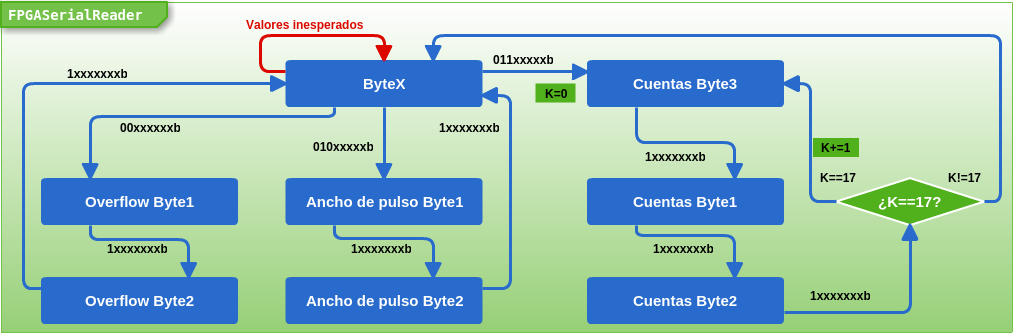
\includegraphics[keepaspectratio, width=1\textwidth]{./img/reader.png}
		\caption{Máquina de Moore. \texttt{FPGASerialReader}.}   
		\label{fig:reader}
	\end{figure}

\section{\texttt{CountsManager}}
	Este módulo software se encarga de recolectar la información que el \texttt{FPGASerialReader} y \texttt{SensorsManager} generan. Seguidamente
	procede a calcular el valor global y las correcciones por presión y efficiencia. Finalmente se encarga de guardar los datos en la base de
	datos local. En la figura \ref{fig:soft_adquisición} podemos ver el diagrama que describe el funcionamineto que acabamos de explicar. A
	continuación procedemos a explicar a fondo estos pasos.
	\subsection{Recolectar información}
		Como vimos en el capítulo \ref{entornoHW}, la FPGA tan sólo transmite los datos de las cuentas cuando estas son solicitadas con el
		comando apropiado. Este módulo es el encargado de mandar el comando al principio de cada minuto. La información transmitida por la
		FPGA es procesada por el \texttt{FPGASerialReader} y almacenada en variables compartidas accesibles por el \texttt{CountsManager}.
		Después de mandar el comando apropiado para solicitar las cuentas este \emph{thread} se queda esperando hasta que el
		\texttt{FPGASerialReader} le notifique que las cuentas han sido enviadas y procesadas. Al ser notificado este módulo procede a leer de
		las variables compartidas donde está almacenada la información de las cuentas. Dicha notificación se realiza mediante un
		\texttt{threading.Lock}
		\par
		Los valores de presión atmosférica, diferencia de potencial generado por las fuentes de alimentación y temperatura ambiente son
		obtenidos haciendo uso del \texttt{SensorsManager}, que será descrito en secciones futuras de este capítulo.
	\subsection{Median Algorithm y Correcciones}
		Como hemos comentado al principio de esta sección este módulo calcula el valor global y una serie de correcciones sobre este. El valor
		global es una representación de las mediciones de todos los tubos, algo como una media. En el capítulo \ref{cap1} explicamos la
		necesidad de este valor, en este vamos a explicar el algoritmo que es utilizado para calcularle.
	  	\par 
		El MedianAlgorithm\cite{MedianAlgr} tiene dos entradas, un vector con las cuentas actuales de cada canal y un segundo vector con la
		media de cuentas para cada canal. Este vector con cuentas medias es calculado durante un intervalo temporal en el que la presión
		atmosférica no fluctúa y además esta se corresponde al valor medio de presión para la estación. Además es deseable que durante dicho
		intervalo no ocurran eventos que pueden afectar la cantidad de partículas que llegan al instrumento. Este vector de valores medio es
		especificado  en el archivo de configuración que previamente discutimos por lo que es fácilmente modificable. El algoritmo empieza
		calculando la desviación relativa sobre la media de cada canal, los canales con una desviación grande son descartados. Comparando la
		desviación de los canales restantes seleccionamos el mediano, de aquí el nombre del algoritmo. La desviación relativa del canal
		seleccionado es multiplicada por el sumatorio del vector de cuentas medias. El algoritmo devuelve el valor generado por la
		multiplicación. A continuación presentamos la implementación del algoritmo.
		\begin{lstlisting}[style=myPython]
def medianAlgorithm(self, counts):
   # Calculamos la desviación sobre la media.
   r=[x/z for x,z in zip(counts, self.channel_avg) 
      # Descartamos los canales con desviación grande.
      if z>0 and (x/z)>0.3 and (x/z)<10]
   tet = numpy.median(r)
   s0  = sum(self.channel_avg)
   return s0*tet
		\end{lstlisting}
		\par 
		Una vez calculado el valor global usando el MedianAlgorithm procedemos a calcular las dos correcciones. La primera es la corrección
		por presión. Como explicamos en el cápitulo \ref{cap1} la presión atmosférica influye en el proceso de adquisición. Para realizar la
		corrección por presión hay dos factores que se toman en cuenta. El primero es la desviación de la presión actual respecto al valor
		medio de presión para la estación. El segundo es el coeficiente de correlación de los tubos respecto a la presión atmosférica. Este
		coeficiente ha sido calculado por el equipo de CaLMa, siendo el método utilizado desconocido para el autor de este trabajo. En la
		ecuación \ref{eq:pression} podemos ver como se usan estos dos factores, donde $N_0$ es el valor sin corregir, $N$ el valor corregido,
		$\beta$ el coeficiente de corelación, $P$ la presión actual y $P_0$ la presión media para la estación.
		\begin{equation}\label{eq:pression}
		  N=N_0*exp(\beta*(P-P_0))
		\end{equation}
		La segunda corrección que realizaremos es la corrección por eficiencia. Esta es una corrección muy simple, consiste en aplicar un
		factor multiplicativo a la corrección por presión. Esta corrección se puede ver en la fórmula \ref{eq:efficiencia}, donde $N_0$ es el
		valor de la corrección por presión, $N$ el valor de la corrección por eficiencia y $\gamma$ el factor de corrección. 
		\begin{equation}\label{eq:efficiencia}
		  N=N_0*\gamma
		\end{equation}
		Cambios en el entorno de la estación pueden causar cambios en la cantidad de eventos medidos, por ejemplo las precipitaciones de nieve
		pueden reducir la cantidad de partículas que llegan al instrumento. Una persona que analiza los datos con propósito científico puede
		equívocamente asociar el decremento con algún fenómeno físico, mientras que este es debido a un fenómeno técnico.  Este problema es
		solventado con la corrección por eficiencia.   
	\subsection{Base de datos}
		Como ya hemos explicado los datos son guardados en una base de datos para cuya gestión utilizamos \emph{Sqlite3}. En la base de datos tenemos
		tres tablas que a continuación procedemos a explicar.
	    	\par
		La primera tiene el nombre de \texttt{binTable}, nombre que hemos heredado de los primeros sistemas de adquisición rusos. En esta
		guardamos la información de las cuentas de cada minuto. Junto a las cuentas guardamos la fecha y hora en los que se realizó la medida,
		la lectura del barómetro y la lectura de las fuentes de alta tensión.
	    	\par 
		En la segunda tabla llamada \texttt{CALM\_ori}, nombre definido por el NMDB, guardamos el valor global y sus correcciones.  Junto a
		estos valores también guardamos el valor de la fecha y hora en los que se realizó la medida, y también el valor de la presión
		atmosférica.
	    	\par
		En la última tabla guardamos los valores de los anchos de pulsos. Dado al gran número de pulsos, guardar la información de cada uno
		por separado no es práctico. Para ilustrar el problema pondremos de ejemplo la estación de CaLMa donde son procesados unos 4500 pulsos
		cada minuto, siendo esta una de las estaciones con menos eventos por minuto debido a su baja latitud.  Para sobrevenir este problema
		construimos un histograma que guardamos en la base de datos, en forma de cadenas JSON\cite{JSON}. Los histogramas se construyen con
		los datos de diez minutos, intervalo que marca la resolución de los datos de esta tabla.

\section{\texttt{DBUpdater}}
	Este módulo software es el encargado de actualizar el contenido de la base de datos remota. El funcionamiento de este es muy simple y se puede
	ver en la figura \ref{fig:soft_adquisición}. Empieza estableciendo la conexión con la base de datos remota. Si esta se establece se procede a
	leer la última entrada en la base de datos remota. Seguidamente el software calcula la diferencia entre las dos bases de datos, para este
	propósito usa la fecha y hora de la entrada leída de la base de datos remota. Finalmente el software selecciona las diferencias entre las dos
	bases de datos y las escribe en la remota. Es entonces cuando la ejecución de este \emph{thread} termina.  A fin de asegurar la sincronización
	en tiempo real se crea y lanza una instancia de este \emph{thread} cada minuto.
	\par
	Si la conexión con la máquina que alberga a la base de datos remota se pierde por un tiempo, cuando esta vuelva a restablecerse el
	\texttt{DBUpdater} sincronizará las dos bases de datos. Eventualmente si las diferencias entre las dos bases de datos son muy grandes la
	sincronización no ocurre de golpe, de esta manera evitamos sobrecargar al sistema.

\section{\texttt{SensorsManager}}
	Este es el módulo software encargado de manejar los sensores. Por sensores nos referimos al barómetro, las fuentes de alta tensión o los
	termómetros si están presentes. A este módulo se le pasa la información referente a los sensores desde el archivo de configuración. De acuerdo
	con esta información este módulo invoca las funciones de configuración necesarias. Una vez realizada esta configuración inicial podemos
	empezar a leer la información de los sensores. Para este propósito este módulo exporta tres funciones, que se explican a continuación.
	\subsection{Presión atmosférica}
		Para leer el valor actual de la presión atmosférica este módulo nos ofrece la función \texttt{read\_pressure}. Si en el archivo de
		configuración hemos especificado que no tenemos barómetro esta función devuelve un \emph{-1}, así como en el caso de que se produzca
		algún error. Actualmente se soportan dos tipos de barómetros, el \emph{BM35} y el \emph{AP1}. La lógica para manejar estos dos
		barómetros se encuentra en los archivos \texttt{BM53Driver} y \texttt{AP1Driver} respectivamente. No explicaremos a fondo el
		funcionamiento de estos dos. Tan solo destacaremos que el \emph{BM35} se comunica mediante un puerto serie y el \emph{AP1} mediante
		tres señales digitales que son reloj, \emph{strobe} y datos.
	\subsection{Fuentes de alta tensión}
		En el caso de las fuentes de alta tensión las tenemos de dos tipos, analógicas y digitales. Las digitales transmiten su información
		mediante un puerto serie. Las analógicas mediante una señal analógica entre 0V y 5V, que es proporcional a la tensión ofrecida por la
		fuente. La lógica para operar con las fuentes analógicas está en el archivo \texttt{HVPSDriver}, la lógica para las fuentes digitales
		no está implementada porque no hemos podido trabajar con estas. Eventualmente si se produce algún error se devuelve el valor de
		\emph{-1}.
	\subsection{Temperatura}
		Como hemos comentado en muchas estaciones la temperatura ambiente es monitorizada también. Este no es el caso de CaLMa, razón por la
		que no hemos escrito ningunos drivers. Sin embargo el código está pensado para poder ser fácilmente ampliado en caso de necesidad. 

\section{Pruebas unitarias}
	Durante la realización de este trabajo hemos escrito una serie de test unitarios\cite{UnitTest}. Los test unitarios son una técnica que
	permite comprobar el funcionamiento correcto de pequeños módulos o funciones. Las pruebas unitarias a diferencia de otras técnicas pueden ser
	usadas desde una etapa muy inicial del proyecto, incluso existen metodologías como \emph{Desarrollo dirigido por pruebas} donde las pruebas
	son escritas primero y después es escrita la función que pasa la prueba. Recalcamos que en este trabajo no hemos seguido esta metodología.
	\par
	Para que las pruebas unitarias sean aplicables es necesario que el código este bien estructurado. Un código con funciones pequeñas donde cada
	función tiene un propósito bien definido es fácil de testear. El simple hecho de poder escribir un test de una función indica que dicha
	función está bien estructurada. Escribir pruebas unitarias conlleva refactorizar el código, haciéndolo mejor.
	\par
	Las pruebas unitarias son muy útiles y es recomendable que estas tengan una gran cobertura, pero no siempre es posible escribir pruebas
	unitarias para todas las funciones. Pongamos como ejemplo una función que lee una entrada desde una base de datos. Aunque la función este bien
	estructurada es difícil testearla por múltiples razones. Por ejemplo el valor devuelto depende de los datos presentes en la base de datos,
	suponiendo que esta está presente y está configurada correctamente. Es difícil escribir pruebas unitarias para este tipo de funciones, razón
	por la que existen las pruebas de integración.
	\par
	Para realizar los test unitarios hemos utilizado \emph{mocks}(objetos simulados). Estos son objetos que simulan el comportamiento de objetos
	reales de una forma controlada. Por ejemplo en nuestra aplicación hemos utilizado un \emph{mock} para simular el comportamiento de los puertos
	serie. Veamos un pequeño ejemplo donde comprobamos la función \texttt{FPGASerialReader.run()}, función que es encargada de interpretar los
	datos que llegan por la UART de pulsos desde la FPGA.
	\begin{lstlisting}[style=myPython]
def test_high_level_pulse(self):
   port=MagicMock()
   port.inWaiting.return_value=1
   # Secuencia de bytes que representan un mensaje de
   # ancho de pulso.
   port.read.side_effect= \
        ReturnSequence([['\x43'],['\x80'],['\xA0']],None)	

   reader=FPGASerialReader(port, None, [], [], [])
   reader.run()
   self.assertEqual(reader.shared_countsFromEvents[3],1)
#------------------------------------------------------
class ReturnSequence(object):
   def __init__(self, return_sequence, expired):
      self.return_sequence = return_sequence
      self.expired = expired
   def __call__(self, *args):
      if 0  < len(self.return_sequence):
         return self.return_sequence.pop(0)
      else:
         return self.expired
	\end{lstlisting}
	\par
	El objeto \texttt{port} es el objeto que representa el puerto como vemos este es un \emph{mock}. La función \texttt{inWaiting} que devuelve el
	número de datos disponibles es configurada para que siempre devuelva \texttt{1}. La función \texttt{read} es configurada para devolver
	múltiples valores en un orden concreto. Seguidamente es creado el objeto cuya función queremos probar pasándole la referencia del \emph{mock}, una
	vez creado invocamos la función \texttt{run}. Finalmente comprobamos si el atributo \texttt{shared\_countsFromEvents} tiene el valor esperado.
	\par
	En el ejemplo anterior hicimos la comprobación sobre el valor de un atributo con la función \texttt{assertEqual()}. Los \emph{mocks} ofrecen
	aún más funcionalidad, las funciones \texttt{assert\_called\_with()} y \texttt{assert\_has\_calls()} que permiten comprobar las llamadas que
	han sido realizadas sobre los \emph{mocks}.
	\par
	Junto a las pruebas unitarias hemos utilizado la biblioteca \texttt{coverage} que permite medir la cobertura de estas. Una mayor cobertura
	siempre es mejor, pero no debe convertirse en un objetivo principal. Como hemos dicho para ciertas funciones, como las que interactúan con una
	base de datos es difícil concebir una prueba unitaria. En la figura \ref{fig:coverage} presentamos el resumen de cobertura generado por
	\texttt{coverage}. Podemos ver que las pruebas para el \texttt{CountManager} no son muy extensas debido a que este es un módulo que interactúa
	mucho con las bases de datos. Sin embargo podemos ver que la cobertura del \texttt{DBUpdater} es del 100\%, esto es debido a que los test
	escritos para este módulo no son unitarios, esto son más bien test de integración. Durante el proceso de implementación surgió la necesidad de
	estos, razón por la que son incluidos en este trabajo.
	\begin{figure}[h]
		\centering
		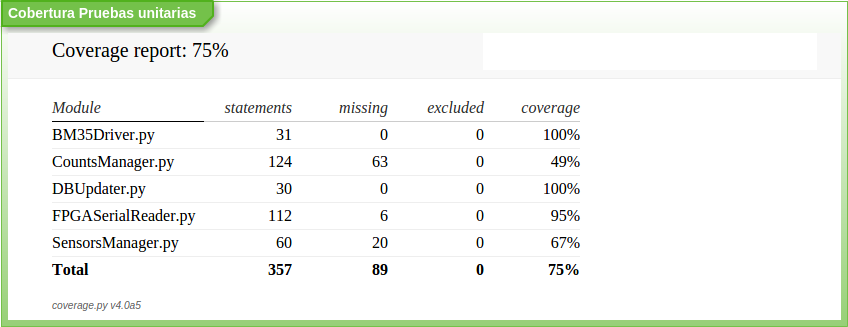
\includegraphics[keepaspectratio, width=1\textwidth]{./img/coverage.png}
		\caption{Cobertura Pruebas unitarias}   
		\label{fig:coverage}
	\end{figure}
